\documentclass[10pt,a5paper]{extarticle}
\usepackage[margin=.8cm,bottom=10mm]{geometry}
\usepackage[utf8]{inputenc}
\usepackage[IL2]{fontenc}
\usepackage[czech]{babel}
\usepackage{microtype}
\usepackage{amssymb}
\usepackage{amsthm}
\usepackage{amsmath}
\usepackage{xcolor}
\usepackage{graphicx}
\usepackage{wasysym}
\usepackage{multicol}
\usepackage[inline]{enumitem}

\newcommand{\R}{\mathbb{R}}
\newcommand{\N}{\mathbb{N}}

\newcommand{\hint}[1]{{\color{gray}\footnotesize\noindent(Nápověda: #1)}}

\setlist[enumerate]{label={(\alph*)},topsep=\smallskipamount,itemsep=\smallskipamount,parsep=0pt,itemjoin={\quad}}
\setlist[itemize]{topsep=\smallskipamount,noitemsep}

\def\tisk{%
\newbox\shipouthackbox
\pdfpagewidth=2\pdfpagewidth
\let\oldshipout=\shipout
\def\shipout{\afterassignment\zdvojtmp \setbox\shipouthackbox=}%
\def\zdvojtmp{\aftergroup\zdvoj}%
\def\zdvoj{%
    \oldshipout\vbox{\hbox{%
        \copy\shipouthackbox
        \hskip\dimexpr .5\pdfpagewidth-\wd\shipouthackbox\relax
        \box\shipouthackbox
    }}%
}}%

\let\results\newpage
\let\endresults\relax

\def\resultssame{%
    \long\def\results##1\endresults{%
        \vfill
        \noindent\rotatebox{180}{\vbox{##1}}%
    }%
}


\newtheorem*{poz}{Pozorování}

\theoremstyle{definition}
\newtheorem{uloha}{\atr Úloha}
\newtheorem{suloha}[uloha]{\llap{$\star$ }Úloha}
\newtheorem*{bonus}{Bonus}
\newtheorem*{defn}{Definice}

\pagestyle{empty}


\let\ee\expandafter

\def\vysld{}
\let\printvysl\relax
\let\printalphvysl\relax

\makeatletter
\long\def\vyslplain#1{\ee\ee\ee\gdef\ee\ee\ee\vysld\ee\ee\ee{\ee\vysld\ee\printvysl\ee{\the\c@uloha}{#1}}}
\let\vysl\vyslplain

\def\locvysl#1{\ee\gdef\ee\locvysld\ee{\locvysld\item #1}}
\let\lv\locvysl

\newenvironment{ulohav}[1][]{\begin{uloha}[#1]\gdef\locvysld{\begin{enumerate*}}}{\ee\vyslplain\ee{\locvysld\end{enumerate*}}\end{uloha}}
\def\stitem{\@noitemargtrue\@item[$\star$ \@itemlabel]}

\makeatother

\def\atr{}
\def\basic{\def\atr{\llap{\mdseries$\sun$ }\gdef\atr{}}}
\def\interest{\def\atr{\llap{$\star$ }\gdef\atr{}}}
\def\iinterest{\def\atr{\llap{$\star\star$ }\gdef\atr{}}}


\def\st{^\circ}

\begin{document}

% \tisk
% \resultssame

\section*{14. Orientované úhly, oblouková míra}

\begin{ulohav}
Převeďte na radiány:
\begin{enumerate}
    \item $135^\circ$, $150^\circ$, $210^\circ$, $240^\circ$, $330^\circ$, $360\st$, $450^\circ$, $1200\st$, $-60\st$ \lv{$\frac{3 \pi }{4}$, $\frac{5 \pi }{6}$, $\frac{7 \pi }{6}$, $\frac{4 \pi }{3}$, $\frac{11 \pi }{6}$, $2\pi$, $\frac52\pi$, $\frac{20}3\pi$, $-\frac\pi3$}
    \item $12\st30'$, $36\st10'$, $145\st$, $317\st18'$ \lv{$\frac{5 \pi }{72},\frac{217 \pi }{1080},\frac{29 \pi }{36},\frac{3173 \pi }{1800}$, zaokrouhleně $0{,}218166$, $0{,}631227$, $2{,}53073$, $5{,}53793$}
\end{enumerate}
\end{ulohav}

\begin{uloha}
Převeďte na stupně z radiánů: $\frac43\pi$, $\frac45\pi$, $\frac{12}5\pi$, $\frac{14}9 \pi$, $\frac7{10}\pi$, $\frac1{15}\pi$, $3\pi$, $10\pi$, $-\pi$
\vysl{$240\st$, $ 144\st$, $ 432\st$, $ 280\st$, $ 126\st$, $ 12\st$, $ 540\st$, $ 1800\st$, $ -180\st$}
\end{uloha}



\begin{ulohav}
Určete základní velikosti úhlů
\begin{enumerate}
    \item $270\st$, $ 425\st$, $ 1607\st$, $ 2527\st$, $ 2550\st$, $ 2667\st$, $ 2711\st$, $ 3312\st$, $4683\st$, $1000\st30'$
        \lv{$270\st$, $ 65\st$, $ 167\st$, $ 7\st$, $ 30\st$, $ 147\st$, $ 191\st$, $ 72\st$, $ 3\st$, $280\st30'$}
    \item $-6\st$, $-175\st$, $-670\st$, $-872\st$, $-937\st$,
        \lv{$354\st$, $185\st$, $50\st$, $208\st$, $143\st$}
    \item $\frac{\pi }{3}$, $\frac{5 \pi }{4}$, $\frac{7 \pi }{3}$, $11 \pi $, $20 \pi $, $\frac{20 \pi }{3}$, $\frac{50 \pi }{13}$, $777 \pi $, $9000 \pi$ 
        \lv{$\frac{\pi }{3}$, $\frac{5 \pi }{4}$, $\frac{\pi }{3}$, $\pi $, $0$, $\frac{2 \pi }{3}$, $\frac{24 \pi }{13}$, $\pi $, $0$}
    \item $-\pi $, $-2 \pi $, $-\frac{\pi }{3}$, $-\frac{2}{5} \pi$, $-\frac{3}{2} \pi$, $-\frac{7}{2} \pi $, $-13 \pi $, $-20 \pi $, $-\frac{20}{3} \pi $
        \lv{$\pi $, $0$, $\frac{5 \pi }{3}$, $\frac{8 \pi }{5}$, $\frac{\pi }{2}$, $\frac{\pi }{2}$, $\pi $, $0$, $\frac{4 \pi }{3}$}
\end{enumerate}
\end{ulohav}

\begin{uloha}
Určete přesné hodnoty funkcí sin, cos, tg, cotg pro $30\st$, $45\st$ a $60\st$. \hint{Pro $30\st$ a $60\st$ použijte rovnostranný trojúhelník.}
\vysl{\begin{tabular}{c|c|c|c|c}
 & sin & cos & tg & cotg \\ \hline
$30\st$ & $\frac12$ & $\frac{\sqrt3}2$ & $\frac{\sqrt3}3$ & $\sqrt3$ \\ \hline 
$45\st$ &  $\frac{\sqrt2}2$ & $\frac{\sqrt2}2$ &  1 & 1 \\ \hline 
$60\st$ & $\frac{\sqrt3}2$ & $\frac12$ & $\sqrt3$ & $\frac{\sqrt3}3$
\end{tabular}}
\end{uloha}


\interest
\begin{uloha}
Zdůvodněte, proč platí vztah $\sin^2 x + \cos^2 x = 1$.
\end{uloha}

\interest
\begin{uloha}
S pomocí následujícího obrázku určete přesnou hodnotu $\operatorname{tg} 22{,}5\st$.
\[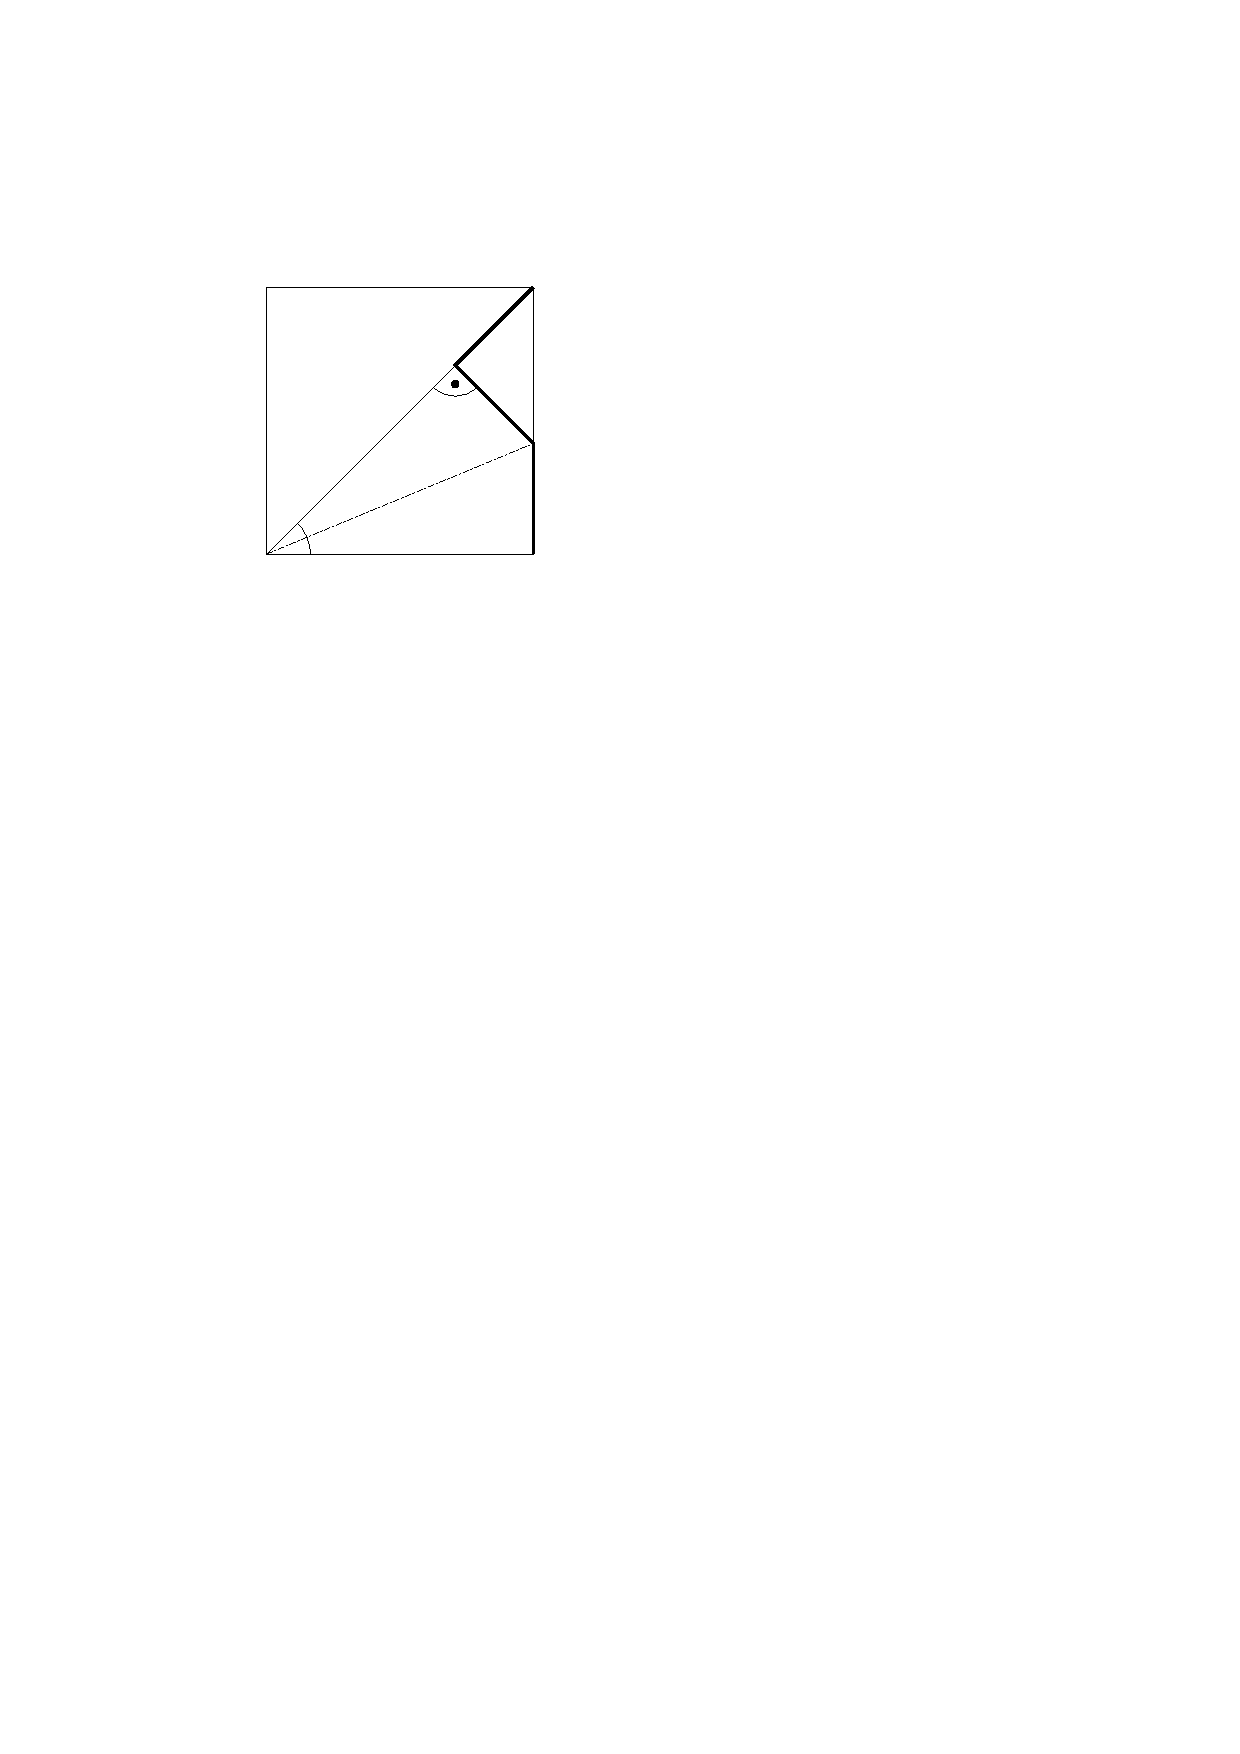
\includegraphics{sinpi8.pdf}\]
\end{uloha}


\results
\parindent=0pt
\parskip=\smallskipamount
\rightskip=0pt plus1fil\relax
\def\printvysl#1#2{\textbf{#1.} #2\par}
\vysld
\endresults


\end{document}